\documentclass{beamer}
%\usepackage{beamerarticle}
\usepackage{heppennames}
\usepackage{hepnicenames}
\usepackage{graphicx} 
\usepackage{multirow}
\usepackage{amsbsy,amsmath,amssymb}
\usepackage{booktabs}
% ********** Styl prezentacji **********
\mode<presentation>
{
	\usetheme{Singapore}
  \setbeamercovered{transparent}
   \setbeamertemplate{footline}[frame number] 
  \setbeamertemplate{navigation symbols}{ 
  \insertslidenavigationsymbol
  \insertframenavigationsymbol
  \insertsubsectionnavigationsymbol
  \insertsectionnavigationsymbol
  \insertdocnavigationsymbol
  \insertbackfindforwardnavigationsymbol
  \hskip 0.3cm
  %\insertframenumber / \inserttotalframenumber  % <<< frame #
  %\insertpagenumber / \insertpresentationendpage % <<< page #
} 
}

\usepackage[english]{babel}
\usepackage[latin1]{inputenc}

% font definitions, try \usepackage{ae} instead of the following
% three lines if you don't like this look
\usepackage{mathptmx}
\usepackage[scaled=.90]{helvet}
\usepackage{courier}


\usepackage[T1]{fontenc}
\author{S. Poss, \emph{C.B. Lam, J. Strube, C. Grefe}}
\institute[CERN]{CERN}

\subject{CLICProduction}
\AtBeginSubsection[]
{
	\begin{frame}<beamer>
		\frametitle{Outline}
		\tableofcontents[currentsection,currentsubsection]
	\end{frame}
}

\title[]{Monte Carlo production for the CLIC CDR}
\subtitle{Our experience}

\date{\today}

\begin{document}

\begin{frame}
	\titlepage
\end{frame}

\begin{frame}
	\frametitle{Table of contents}
	\begin{itemize}
\item Introduction
\item Production framework
\item CLIC productions
\item Prospects
\item Conclusion
\end{itemize}
\end{frame}

\section{Introduction}

\begin{frame}
	\frametitle{Introduction}
\begin{itemize}
\item 6 benchmark analysis: 
\begin{itemize}
\item $\Pep\Pem \to \Ph \Pgne \Pagne$,
\item  $\Pep\Pem \to \PHp \PHm$, $\Pep\Pem \to \PHz \PA$, 
\item $\Pep\Pem \to \PSq_R \PaSq_R$, 
\item $\Pep\Pem \to \PSl \PaSl \,(\ell = \Pe,\Pgm)$, 
\item $\Pep\Pem \to \PSgxpm_i \PSgxmp_j,\, \Pep\Pem \to \PSgxz_i \PSgxz_j$,
\item  $\Pep\Pem \to \Pqt \Paqt$ (500~GeV).
\end{itemize}
\item Plus all the backgrounds (Standard Model)
\item 2 detector models
\end{itemize}
Number of events processed in the last 9 months: $17\cdot 10^6$ generated, $29\cdot 10^6$ simulated, $17\cdot 10^6$ reconstructed.
\end{frame}

\part{Framework}
\begin{frame}
\partpage 
\end{frame}

\section{Production framework}
\begin{frame}
	\frametitle{Production framework}
DIRAC has a Transformation System:
\begin{itemize}
\item  Create a work flow object (XML representation of a job), and let the system create the jobs for you
\item Productions are identified with a unique ID
\item Automatic resubmission of failed jobs: minor monitoring needed
\end{itemize}
~\\
It \alert{saved us a huge amount of time and man power}.
\end{frame}

\begin{frame}
\frametitle{Production framework}
The DIRAC transformation system comes with a useful set of API commands: get properties, change them, update inputs, etc.\\
~\\
\alert{Full interface to the ILD and SiD software frameworks}, and to WHIZARD and PYTHIA code. Additionally we have an interface for generator level cuts (StdhepCut tool from Lars Weuste), Overlay input, etc.~\\

\end{frame}

\begin{frame}
\frametitle{Defining steps}
\begin{itemize}
\item Decided to split all steps in different jobs, implying specific productions for:
\begin{itemize}
\item Generation: WHIZARD/PYTHIA.
\item Simulation: Mokka/SLIC.
\item Reconstruction: Marlin/LCSIM-SLICPandora-LCSIM.
\end{itemize}
\item Because of long simulation and reconstruction CPU time, few number of events per step ($10-50$) are required $\Rightarrow$ small files to manage.
\item Chaining of productions is straightforward, more on that later: \alert{data driven production management}.
\end{itemize}
All files produced are stored in the DIRAC replica and Metadata catalog
\end{frame}

\section{Replica Catalog and Metadata catalog}
\begin{frame}
\frametitle{Replica catalog} 
\begin{itemize}
\item \alert{DIRAC provides a catalog}: fast and efficient
\item Has the possibility to \alert{write and read in the Lcg FC via the same interface}.
\end{itemize}
In the futur (coming month), when adding a file in the DIRAC FC, it will also enter in the ILC LFC.
 \end{frame}
\begin{frame}
\frametitle{Metadata catalog}
\begin{itemize}
\item ILC stores the metadata encoded in the file names.
\item Somehow restricts the number of meta info that one can add to a given file once the file is created.
\item DIRAC FC comes with a metadata catalogue, that sets the \alert{metadata at directory level} (e.g. production ID, software packages, cross section, polarisation, etc.) and at File level (number of events, etc.).
\item Flexible as one can add (and remove) metadata on the fly.
\item Searchable: find EvtType=tt Datatype=SIM
\item Possibility to set ACLs.
\item Also comes with convenient API commands.
\end{itemize} 
Web interface is under development, should be available for tests in the coming weeks.
 \end{frame}
\section{Monitoring}
\begin{frame}
\frametitle{Production Monitoring}
Monitoring done with web site: 
\begin{itemize}
\item Overview of production statuses: \% of the files processed,\\ failure rate
\item Control of jobs from a given production in two clicks
\item Monitoring and accounting plots also available
\end{itemize}

\end{frame}

\part{CLIC Production}
\begin{frame}
\partpage 
\end{frame}

\section{Production}
\begin{frame}
\frametitle{Defining a production} 
\begin{enumerate}
\item Define the input data (if any) via a metadata query (e.g. meta['ProdID']=186)
\item Define the application and versions you want to use
\item Define the output files and output storage
\end{enumerate}
\alert{Data driven procedure}: if new files are added to the catalogue that correspond to the metadata query, jobs processing those files are automatically created.
\end{frame}


\section{Generation}
\begin{frame}
\frametitle{Generating Events}
Use WHIZARD 1.95 (PYTHIA 6.4) for most samples:
\begin{itemize}
\item Handling of \alert{beam spectrum and ISR included}
\item Adding a \alert{new process} is straight forward
\item Does the correct computation of diagrams and interference: \alert{accurate cross section and phase space}
\item Limitation: \alert{final states have no width}, cannot do $\Pqt\Paqt$, $\PWp\PWm$ or $\PZz\PZz$.
\end{itemize} 
Use PYTHIA 6.4 for those 3 samples:
\begin{itemize}
\item Final states have the correct width
\item Less accurate estimation of cross section and phase space, but compatible to those produced by WHIZARD
\item Has \alert{beam spectrum interface via CALYPSO}, ISR is PYTHIA default
\item Limitation: \alert{less flexibility}, adding a channel cannot be done easily
\end{itemize}
\end{frame}

\section{Simulation}
\begin{frame}
\frametitle{Simulation}
Define productions for both detector concepts, but very similar interface. Not an issue in the production framework:\\
\begin{center}
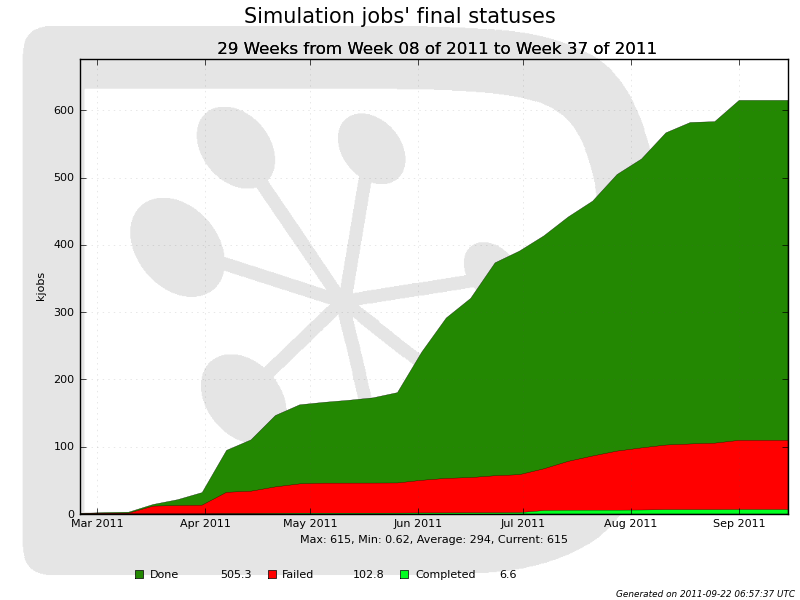
\includegraphics[width=9cm]{SimJobStatus}
\end{center}
\end{frame}

\section{Reconstruction with Overlay}
\begin{frame}
\frametitle{Reconstruction}
 As for the simulation: dedicated productions are created, automatically using files produced by the simulation step.\\
~\\
Without Overlay:\\
\begin{center}
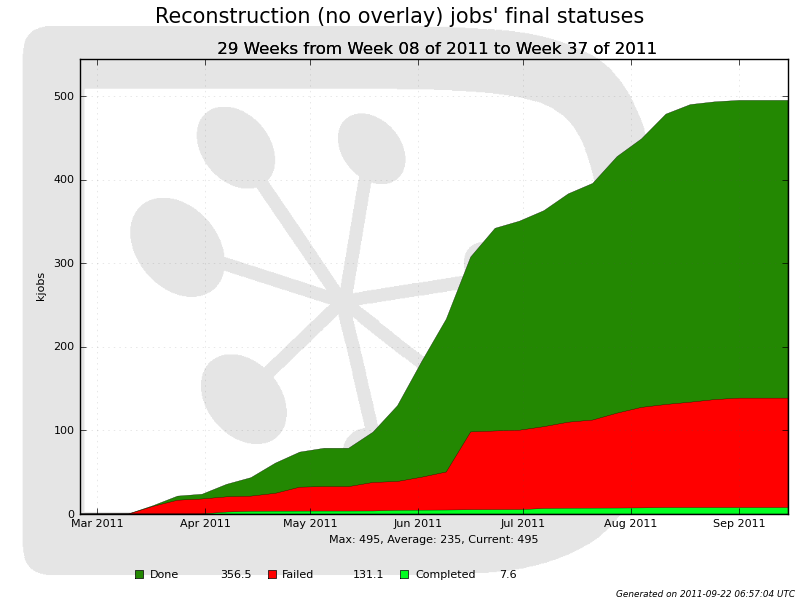
\includegraphics[width=7cm]{RecoNoOverlayStatus}
\end{center}
\end{frame}
\begin{frame}
\frametitle{Reconstruction with overlay}
\begin{center}
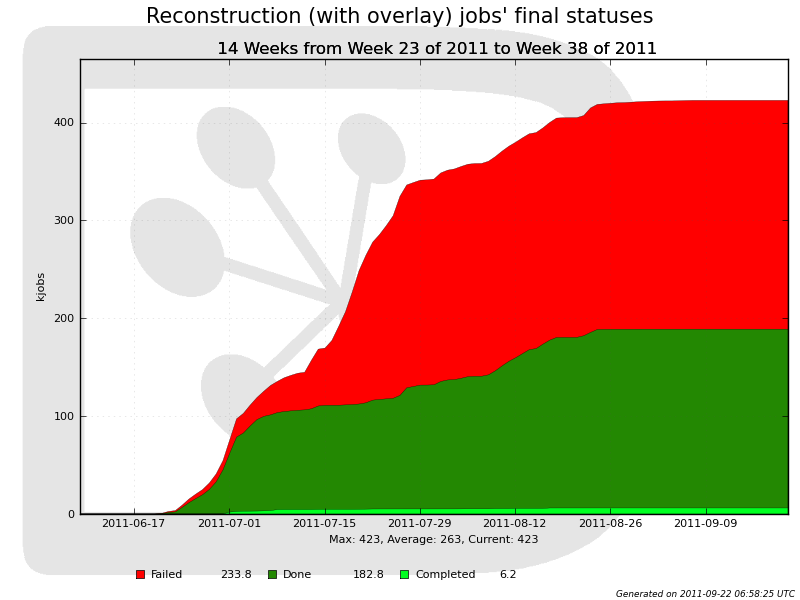
\includegraphics[width=9cm]{RecoOverlayStatus} 
\end{center}
\end{frame}
\begin{frame}
\frametitle{Overlay handling (1)}
CLIC detector benchmark require to reconstruct the physics events with overlaid $\gamma\gamma \to had$ background. \alert{60 BX with 3.2 interactions per BX are considered for every signal event}.\\
~\\
Simulated background files contain $100$ events each (more would be better but CPU is a constrain). For a 10 physics events file, one need $\sim 2000$ bkg events, or \alert{$20$ files per job}.
\end{frame}
\begin{frame}
\frametitle{Overlay handling (2)}
This did not work: storages (CERN in particular, but also IN2P3) do not cope with such a load (2000 jobs trying to access 20 random files each represent a huge number of queries).\\
Solution: \alert{merge the files randomly once} to reduce the number of files needed: merge them by groups of 200 files.\\ 
~\\
Works but requires manual intervention, and one needs a \alert{very large number of files} to have enough combinations.\\
~\\
Needed solution: \alert{use random access} (LCIO v1.51 has it, but not LCSIM). Then only one big file is needed on every site with direct access. No more transfers are needed.
\end{frame}


\part{Prospects}
\begin{frame}
\partpage 
\end{frame}

\begin{frame}
\frametitle{Prospects} 
Now running in the US sites: need to see for disk space. CERN disk requests will be made: for the moment, only 40Tb are available on disk (all used, but as mush as needed on TAPE though).\\
~\\
Will finish implementing dedicated service that will know the available processes, to easy users' lives. For the moment, a text file holds all the processes available and the corresponding WHIZARD version.\\
~\\
Will push to get the File Catalog web browser.
\end{frame}

\part{Conclusion}
\begin{frame}
\partpage 
\end{frame}

\begin{frame}
\frametitle{Conclusion} 
\begin{itemize}
\item $\approx 60$ million events processed in 9 months
\item Used $2\cdot 10^{10}$ KSI2K seconds of CPU in $\sim 20$ sites
\item Data produced correspond to $\sim 130$~TB
\item Most issues were due to storage access (overlay in particular), not to software
\end{itemize}
Overall worked well $\rightarrow$ \alert{CDR is out!}\\
https://edms.cern.ch/document/1160419
\end{frame}

\appendix
\part{Backup slides}
\begin{frame}
\partpage 
\end{frame}
\section{Resources used}
\begin{frame}
\frametitle{Resources used: CPU}
 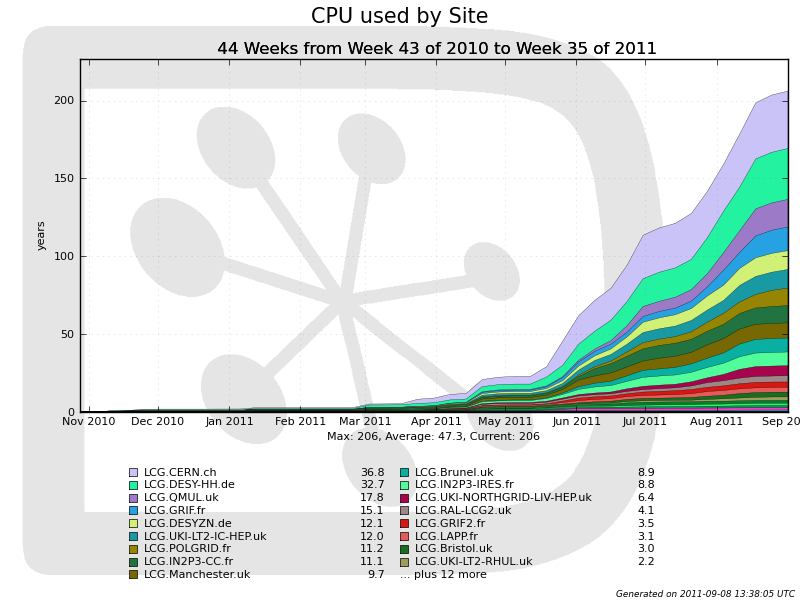
\includegraphics[width=10cm]{CPUperSiteForProd}
\end{frame}
\begin{frame}
\frametitle{Resources used: Storage} 
\begin{center}
\begin{tabular}{crr}
\toprule
Site & Production (TB) & User (TB) \\
\midrule
CERN & 128 & 20\\
IN2P3 & 4 & 9\\
RAL & 4 & 28\\
KEK & 0.02 & 0\\
IMPERIAL& 1.6 & 0 \\
TAU & $4\cdot 10^{-4}$ & 0\\
\bottomrule
\end{tabular}
\end{center}
Sites that can be used in addition: DESY, Bristol, BONN, RALPP
\end{frame}
\section{Technical aspects}
\begin{frame}
\frametitle{Technical aspects}
Dropped pilot mode as some sites did not support it, using private pilot mode\\
~\\
Steering files are installed on the sites like applications (dependency relation), so no need to pass them in the input sandbox of the job.\\
~\\
Software installed in the Shared areas of the sites when/where possible. Does not use SAM framework (yet) as DIRAC takes care of the software installation and removal. 
\end{frame}

\begin{frame}
\frametitle{Services availability}
60 million events correspond to $\sim 4$ million jobs. On average 1000 concurrently running.\\
~\\
File catalog is the most expensive service in terms of CPU and simultaneous queries to DB. Had to duplicate service (not DB). ~\\
~\\
It would be useful to replicate the DB and other services to have more instances available (more VO boxes needed).~\\
~\\
Same problem with JobManager with high load.
\end{frame}

\section{Conventions}
\begin{frame}
\frametitle{File names conventions}
\begin{itemize}
\item Base path is /ilc/prod to separate from /ilc/user data. 
\item Path holds most relevant info (machine, energy, process, detector, data type (gen, SIM, REC, DST), prodID)
\item File name is process\_prodID\_jobID.ext (ext=stdhep,slcio)
\end{itemize} 
 \end{frame}
\section{Data validation}
\begin{frame}
\frametitle{Data validation}
When simulating data with 2 frameworks, it's necessary to validate it before running. For that purpose \alert{TOMATO} was designed: convert the stdhep to slcio (stdhepjob supported by DIRAC), and run TOMATO (Marlin processor) to create histograms of "significant" distributions.  \\
~\\
"Significant" is specific to the different analysis, so every working group needs to provide the variables to be plotted.\\
~\\
Was used for the $\Ptop\APtop$ analysis.
\end{frame}

\end{document}
